\documentclass{article}
% The LaTeX macro language is complicated, so we have inserted
% lots of documenting comments into the file.  Comments start
% with `%' and continue to the end of the line.  In Overleaf's
% window, they are colored green
%
% Comments prefixed with `Student:' are relevant to students.
% Skip anything else you don't understand, or ask me.
%
% set font encoding for PDFLaTeX or XeLaTeX
\usepackage{ifxetex}
\ifxetex
  \usepackage{fontspec}
\else
  \usepackage[T1]{fontenc}
  \usepackage[utf8]{inputenc}
  \usepackage{lmodern}
\fi

% Student: These lines describe some document metadata.
\title{Problem Set 6}
\author{%
% Student: change the next line to your name!
    Name
\\  MATH-UA 120 Discrete Mathematics
}
\date{due December 9, 2022 at 11:00pm}


\usepackage[headings=runin-fixed-nr]{exsheets}
% These make enumerates within questions start at the second ("(a)") level, rather than the first ("1.") level.
\makeatletter
    \newcommand{\stepenumdepth}{\advance\@enumdepth\@ne}
\makeatother
\SetupExSheets{
    question/pre-body-hook=\stepenumdepth,
    solution/pre-body-hook=\stepenumdepth,
}
\DeclareInstance{exsheets-heading}{runin-nn-np}{default}{
    runin = true,
    title-post-code = .\space,
    join = {
        main[r,vc]title[l,vc](0pt,0pt);
    }
}
\newif\ifshowsolutions
% Student: replace `false' with `true' to typeset your solutions.
% Otherwise they are ignored!
\showsolutionsfalse
\ifshowsolutions
    \SetupExSheets{
        question/pre-hook=\itshape,
        solution/headings=runin-nn-np,
        solution/print=true,
        solution/name=Answer
    }%
    \makeatletter%
    \pretocmd{\@title}{Answers to }%
    \makeatother%
\else
    \SetupExSheets{solution/print=false}
\fi

% Bug workaround: http://tex.stackexchange.com/a/146536/1402
%\newenvironment{exercise}{}{}
\RenewQuSolPair{question}{solution}
%\let\answer\solution
%\let\endanswer\endsolution
\usepackage{manfnt}
\newcommand{\danger}{\marginpar[\hfill\dbend]{\dbend\hfill}}

% We are creating a command for some common commands.
\newcommand{\Z}{\mathbb{Z}}
\newcommand{\modulo}{\text{mod }}
\newcommand{\divisor}{\text{ div }}

% This package is for specifying graphics.  It's amazing.
% Manual at http://texdoc.net/texmf-dist/doc/generic/pgf/pgfmanual.pdf
\usepackage{tikz}
\tikzstyle{vertex}=[circle,draw,fill=none,inner sep=0pt,outer sep=0pt, minimum width=1ex]
\tikzstyle{edge}=[draw,thick]
\usepackage{multirow, multicol}
\usepackage{amsmath, amsthm}
\usepackage{amsfonts}
\usepackage{siunitx}
\DeclareSIUnit\pound{lb}
\usepackage{hyperref}
\newtheorem*{theorem}{Theorem}
\theoremstyle{definition}
\newtheorem*{definition}{Definition}
\newenvironment{note}{\noindent\emph{Note}.}{}
% This is the beginning of the part of the file that describes
% the text of the document.
% That's why it says `\begin{document}' below. :-)
\begin{document}
\maketitle



These are to be written up and turned in to Gradescope.\\



\ifshowsolutions
    \SetupExSheets{solution/print=true}
\else
    \danger
 \underline{ \LaTeX  Instructions:}  You can view the source (\texttt{.tex}) file to get some more examples of \LaTeX{} code.  I have commented the source file in places where new \LaTeX{} constructions are used.
  
  Remember to change \verb|\showsolutionsfalse| to \verb|\showsolutionstrue|
    in the document's preamble 
    (between \verb|\documentclass{article}| and \verb|\begin{document}|)
\fi

\section*{Assigned Problems}



\begin{question}
    (Scheinerman, Exercise 35.7:)
    What is wrong with the following statements?  Repair these statements and prove your revised versions.
    \begin{enumerate}
	\item For all integers $a, b$, we have $b \mid a$ iff  $a \divisor b = \frac{a}{b}$.
	\item For all integers $a, b$, we have $b \mid a$ iff $a \bmod b = 0$.
    \end{enumerate}
\end{question}
% Student: put your answer between the next two lines.
\begin{solution}
\end{solution}

\begin{question}
    Find integers $a, b$ that do not have a greatest common divisor.  Prove that the pair of numbers that you found are the only pair of integers that do not have a gcd.
\end{question}
% Student: put your answer between the next two lines.
\begin{solution}
\end{solution}

\begin{question}
    (Scheinerman, Exercise 36.2:)
    For each pair of integers $a$ and $b$, find integers $x$ and $y$
    such that $ax+by = \gcd(a,b)$.
    \begin{enumerate}
        \item $\gcd(20,25)$
        \item $\gcd(0,10)$
        \item $\gcd(-89,-98)$
        \item $\gcd(123,-123)$
        \item $\gcd(54321,50)$
        \item $\gcd(1739,29341)$
    \end{enumerate}
\begin{note}
    You should do all of these for practice.
    But you only need to turn in (a), (c), and (e).
\end{note}
\end{question}
% Student: put your answer between the next two lines.
\begin{solution}
\end{solution}

\begin{question}
    (Scheinerman, Exercise 36.12:) 
    Let $a$ be an integer.  Prove that $2a+1$ and $4a^2+1$ are relatively prime.
\end{question}
% Student: put your answer between the next two lines.
\begin{solution}
\end{solution}


\begin{question}
    (Scheinerman, Exercise 36.20:)
    A class of $n$ children sit in a circle.
    The teacher walks around the outside of the circle and pats every
    $k$th child on the head.
    Find and prove a necessary and sufficient condition on $n$ and $k$
    for every child to receive a pat on the head.
\end{question}
% Student: put your answer between the next two lines.
\begin{solution}
\end{solution}

\begin{question}
     Let $G=(V,E)$ be a graph. Prove by induction: 
\begin{quote}
The sum of the degrees of the vertices in $G$ is twice the number of edges.
\end{quote}	
\end{question}
% Student: put your answer between the next two lines.
\begin{solution}
\end{solution}

\begin{question}
    (Scheinerman, Exercise 47.15:)
    Let $G$ be a graph. Prove that there must be an even number of vertices of odd degree.
\end{question}
% Student: put your answer between the next two lines.
\begin{solution}
\end{solution}

\begin{question}
    Suppose $G$ is a subgraph of $H$.  Prove or disprove:
\begin{enumerate}
	\item $\alpha(G) \leq \alpha(H)$
	\item $\omega(G) \leq \omega(H)$
	\end{enumerate}
\end{question}
% Student: put your answer between the next two lines.
\begin{solution}
\end{solution}


\begin{question}
    (Scheinerman, Exercise 47.21:)
    Let  $G$ and $H$ be graphs.  We say that $G$ is \emph{isomorphic} to $H$
    provided there is a bijection $f \colon V(G) \to V(H)$ such that
    for all $a,b \in V(G)$ we have $a \sim b$ (in $G$) if and only if $f(a) \sim
    f(b)$ (in $H$).  The function $f$ is called an \emph{isomorphism} of $G$ to
    $H$.  We can think of $f$ as renaming the vertices of $G$ with the names of
    the vertices in $H$ in a way that preserves adjacency.  Less formally,
    isomorphic graphs have the same drawing (except for the names of the
    vertices).
    \begin{enumerate}
        \item Prove that isomorphic graphs have the same number of vertices.
        \item Prove that  if $f \colon V(G) \to V(H)$ is an
            isomorphism of graphs $G$ and $H$ and if $v \in V(G)$, then the
            degree of $v$ in $G$ equals the degree of $f(v)$ in $H$.
        \item Prove that isomorphic graphs have the same number of edges.
        \item Give an example of two graphs that have the same number of
            vertices and same number of edges but are not isomorphic.
        \item Let $G$ be the graph whose vertex set is $\{ 1,2,3,4,5,6\}$.  In
            this graph, there is an edge from $v$ to $w$ if and only if $v-w$ is
            odd.  Let $H$ be the graph below.  Find an
            isomorphism $f \colon V(G) \to V(H)$.
    \end{enumerate}
    \begin{center}
    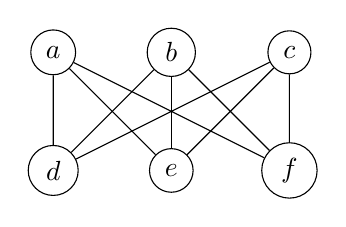
\begin{tikzpicture}[
        every node/.append style={draw,circle}
    ]
        \node (A) at (-1.5, 0) {$a$};
        \node (B) at (0, 0)    {$b$};
        \node (C) at (1.5, 0)  {$c$};
        \node (D) at (-1.5, -1.5) {$d$};
        \node (E) at (0, -1.5)   {$e$};
        \node (F) at (1.5, -1.5) {$f$};
        \draw (A) -- (D) -- (C) -- (F) -- (A);
        \draw (A) -- (E) -- (C);
        \draw (D) -- (B) -- (F);
        \draw (B) -- (E);
    \end{tikzpicture}
    \end{center}
\end{question}
% Student: put your answer between the next two lines.
\begin{solution}
\end{solution}

\begin{question}\label{Sch-48-10}
    (Scheinerman, Exercise 48.10:) Let $G = (V,E)$
    be a graph on with $V = \left\{1,2,3,4,5,6\right\}$.  In
    Figure~\ref{fig-Sch-48-10} we show the graphs $G-1$, $G-2$, and so on but we
    do not show the names of the vertices.
        \begin{figure}\centering
        \begin{tabular}{ccc}
            $G-1$ & $G-2$ & $G-3$ \\
            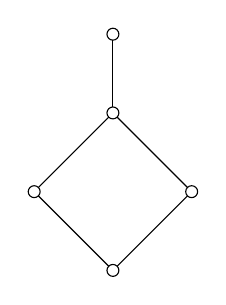
\begin{tikzpicture}
                 \path node[vertex] (A) {}
                     ++ ( 0,-1) node[vertex] (B) {} edge (A)
                     ++ (-1,-1) node[vertex] (C) {} edge (B)
                     ++ ( 1,-1) node[vertex] (D) {} edge (C)
                     ++ ( 1, 1) node[vertex] (E) {} edge (D) edge (B);
            \end{tikzpicture}
            &
            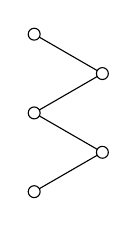
\begin{tikzpicture}
                 \path node[vertex] (A) {}
                     ++ (-30:1) node[vertex] (B) {} edge (A)
                     ++ (-150:1) node[vertex] (C) {} edge (B)
                     ++ (-30:1) node[vertex] (D) {} edge (C)
                     ++ (-150:1) node[vertex] (E) {} edge (D)
                     ;
            \end{tikzpicture}
            &
            \begin{tikzpicture}
                \path node[vertex] (A) {}
                    ++ (0,-1) node[vertex] (B) {} edge (A)
                    ++ (0,-1) node[vertex] (C) {} edge (B)
                    ++ (-1,-1) node[vertex] (D) {} edge (C)
                    ++ (2,0) node[vertex] (E) {} edge (C)
                    ;
            \end{tikzpicture}
            \\[3ex]
            $G-4$ & $G-5$ & $G-6$ \\
            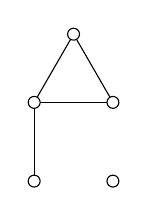
\begin{tikzpicture}
                \path node[vertex] (A) {}
                    ++ (1,0) node[vertex] (B) {} edge (A)
                    ++ (0,-1) node[vertex] (C) {}
                    ++ (-1,0) node[vertex] (D) {} edge (A)
                    (A) ++ (60:1) node[vertex] (E) {} edge (A) edge (B)
                    ;
            \end{tikzpicture}
            &
            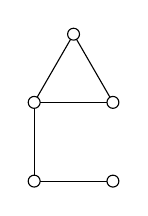
\begin{tikzpicture}
                \path node[vertex] (A) {}
                    ++ (1,0) node[vertex] (B) {} edge (A)
                    ++ (0,-1) node[vertex] (C) {}
                    ++ (-1,0) node[vertex] (D) {} edge (C) edge (A)
                    (A) ++ (60:1) node[vertex] (E) {} edge (A) edge (B)
                    ;
            \end{tikzpicture}
            &
            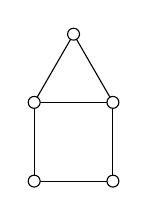
\begin{tikzpicture}
                \path node[vertex,
                    ] (A) {}
                    ++ (1,0) node[vertex,
                    ] (B) {} edge (A)
                    ++ (0,-1) node[vertex,
                    ] (C) {} edge (B)
                    ++ (-1,0) node[vertex,
                    ] (D) {} edge (C) edge (A)
                    (A) ++ (60:1) node[vertex,
                    ] (E) {} edge (A) edge (B)
                    ;
            \end{tikzpicture}
        \end{tabular}
        \caption{$G$ with each of its vertices deleted (Question~\ref{Sch-48-10})}
        \label{fig-Sch-48-10}
    \end{figure}
    The goal of this problem is to reconstruct the original graph $G$. Please do:
    \begin{enumerate}
        \item Determine the number of edges on $G$.
        \item Using your answer to (a), determine the degree of each of the six vertices of $G$.
        \item Determine $G$.
    \end{enumerate}
\end{question}
% Student: put your answer between the next two lines.
\begin{solution}
\end{solution}



\end{document}
